\documentclass[12pt]{article}
\usepackage{enumitem}
%\usepackage[T1]{fontenc}
\usepackage[auth-sc,affil-sl]{authblk}
\usepackage{amsmath}
\usepackage{graphicx}
\usepackage{color}
%\usepackage{enumerate}
\usepackage[round]{natbib}
%\usepackage{url} % not crucial - just used below for the URL 
%\usepackage{amsthm}
\usepackage{amssymb}
\usepackage{graphicx}
\usepackage{epstopdf}
\usepackage{hyperref}
\usepackage{alltt}
\usepackage{listings}
\usepackage{array}
\usepackage[noline, boxed, procnumbered, linesnumberedhidden, titlenumbered]{algorithm2e}
\usepackage[firstpage]{draftwatermark}
\usepackage[margin=1in]{geometry}  %%jcgs has own margins
\usepackage{lmodern}

%\pdfminorversion=4
% NOTE: To produce blinded version, replace "0" with "1" below.
\newcommand{\blind}{0}

\newcommand{\secref}[1]{Section~\ref{#1}}
\newcommand{\tblref}[1]{Table~\ref{#1}}
\newcommand{\figref}[1]{Figure~\ref{#1}}
\newcommand{\thmref}[1]{Theorem~\ref{#1}}
\newcommand{\algref}[1]{Algorithm~\ref{#1}}
\newcommand{\funref}[1]{Function~\ref{#1}}
\newcommand{\listingref}[1]{Listing~\ref{#1}}

\newcommand{\eg}{{\em e.g.}}
\newcommand{\ith}{$i^{th}$}
\newcommand{\cut}[1]{}
\newcommand{\todo}[1]{{\bf\em TODO:} {\em #1}}

\newcommand{\spd}{\fontfamily{cmr}\textsc{\textbf{StratPD}}}

\setlist[enumerate]{itemsep=-1mm}

% DON'T change margins - should be 1 inch all around.
\cut{
\addtolength{\oddsidemargin}{-.5in}%
\addtolength{\evensidemargin}{-.5in}%
\addtolength{\textwidth}{1in}%
\addtolength{\textheight}{1.3in}%
\addtolength{\topmargin}{-.8in}%
}

\begin{document}

\def\spacingset#1{\renewcommand{\baselinestretch}%
{#1}\small\normalsize} \spacingset{1}


%%%%%%%%%%%%%%%%%%%%%%%%%%%%%%%%%%%%%%%%%%%%%%%%%%%%%%%%%%%%%%%%%%%%%%%%%%%%%%

\if0\blind
{
  \title{\bf \spd: A Localized Approach to Partial Dependence Plots for Non-Independent Variables}

  \author{Terence Parr and James Wilson\\
      University of San Francisco\\
}
  \maketitle
} \fi

\if1\blind
{
  \bigskip
  \bigskip
  \bigskip
  \begin{center}
    {\LARGE\bf Title}
\end{center}
  \medskip
} \fi

\bigskip
\begin{abstract}
Pithy abstract here.
\end{abstract}

\noindent%
{\it Keywords:} beer, bbq
%\vfill

%\newpage
%\spacingset{1.5} % DON'T change the spacing!
\section{Introduction}
\label{sec:intro}

In practice, machine learning model interpretation is just as important as obtaining an accurate model. Feature importance is one such interpretation tool, which indicates the relative predictive power of each feature and is helpful when making business decisions. For example, in a model predicting apartment rent prices, the important features often identify what renters are willing to pay for. On the other hand, feature importance does not identify the relationship itself between features (independent variables) $x_i$ and the target (dependent) variable $y$.  Knowing these relationships tells model users a great deal about their data and, indirectly, the associated real-world population. For example, public health officials might be interested in how years of education affect body weight, given a set of observations sampled from a population.

Given just one or two features, a plot of $x_i$ versus $y$ lets us visualize the exact relationship of each feature and $y$.  Because we cannot visualize more than three dimensions, however, this approach does not work for data sets with more than two features.

To get around this limitation, traditional marginal plots project other axes onto the axis associated with the feature of interest.  That means that marginal plots do not isolate the specific contribution of $x_i$ to $y$. For example, a marginal plot of sex (male/female) versus body weight would likely show that, on average, men are heavier than women. While true, men are also taller than women on average, which likely accounts for most of the difference in average weight. It's unlikely that two ``identical'' people, differing only in sex, would be appreciably different in weight.  

As another example, consider the marginal plot of the number of bathrooms versus price shown in \figref{fig:baths_price}(a) (New York City apartment rent data from Kaggle). One would expect a near-linear relationship for the net effect of the number of bathrooms on price, but the marginal plot implausibly suggests that moving from no bathrooms to one bathroom does not affect the price very much.   The apartment prices shown in the marginal plot include the effect of all other features for each apartment.

\cite{PDP} introduced partial dependence (PD) plots as a way to extract and visualize the dependence of $y$ on one or two features of interest. \figref{fig:baths_price}(b) shows the (zero-centered) PD of rent price on the number of bathrooms as a black line. The partial dependence line is the average of the blue lines, which represent the individual conditional expectation (ICE) plots of \cite{ICE}.  In this case, the ICE lines depict the model prediction contributions for a single observation as the bathroom feature shifts through all possible number of bathrooms. Because PD plots represent an average across observations, they can hide a great deal of variability, so it is helpful to combine PD and ICE plots.

\begin{figure}[htbp]
\begin{center}
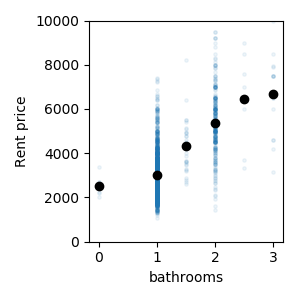
\includegraphics[scale=0.7]{images/baths_vs_price.png}
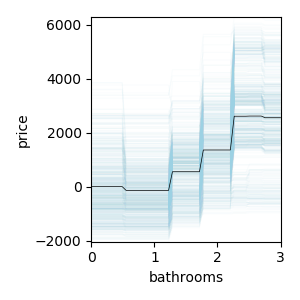
\includegraphics[scale=0.7]{images/baths_vs_price_pdp.png}
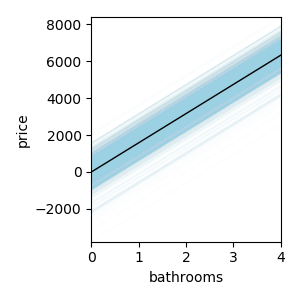
\includegraphics[scale=0.7]{images/baths_vs_price_pdp_lm.png}
\caption{{\bf  Marginal plot and PDP/ICE plot of bathrooms versus rent price}}
\label{fig:baths_price}
\end{center}
\end{figure}

The partial dependence plot largely follows the marginal plot except for the prices of two and three bathroom apartments, where it levels off. This is counterintuitive and exposes an issue with PD and ICE plots. While PD and ICE plots are {\em model-agnostic}, they are not {\em model-independent} and are subject to the strengths and weaknesses of the model making predictions. In \figref{fig:baths_price}(b), the model is a Random Forest(tm) (RF) and RFs cannot extrapolate beyond their support range.  The data set has few apartments with three and four bathrooms, as shown by the lack of blue dots in that range of the marginal plot, so the price predictions appear to flatten out after two bathrooms.  In contrast, \figref{fig:baths_price}(c) shows the PD/ICE plot for the exact same data set but using a linear model (with Lasso regularization).

Getting such radically different PD and ICE plots for different underlying models is undesirable because users cannot distinguish between interesting $y$ curve fluctuations and artifacts of their model choice. At the very least, users should compare plots derived from multiple models. Moreover, PD and ICE plots are only as accurate as the underlying model, meaning PD and ICE plots from derived high-bias models should not be trusted.

There are two remaining issues with PD plots associated with the relationship between features. First, as Friedman pointed out, PD plots are most accurate ``{\em when {\em [the model]} is dominated by low order interactions.}''  Feature interactions such as $x_1x_2$ are difficult to tease apart to obtain partial dependencies on just $x_1$ or $x_2$. ICE plots address this issue by showing separate predicted $y$ curves for each observation as the feature of interest is moved through all possible values.  This not only shows the variation hidden by the PD average curve, but it can depict interaction relationships between the feature of interest and other features. \todo{ref later fig}.

The second issue stems from a lack of independence between features.  In a nutshell, not every combination of dependent features is valid. Consider a five bedroom apartment with just one or even zero bathrooms or a four bathroom studio was no bedroom or an observation identified as male but also pregnant.  Because PD and ICE alter observations by shifting the feature of interest through all possible feature values, they run the risk of conjuring nonsensical observations, and in our experience, features in real data sets are very often dependent to some degree. This problem can be mitigated by computing PD and ICE plots on groups of mutually-dependent or interacting features of interest. \todo{but could involve identifying subsets and computing lots of combinations and we still might want to know about a single contribution.}

To summarize the hazards of PD and ICE plots, both are strongly affected by the model chosen by the programmer.  To obtain accurate plots, PD and ICE rely on the accuracy of the underlying model, which might sacrifice local (\todo{use bold vector x for the first time here?}) accuracy to minimize some global loss function. Both plots use model prediction results rather than the data itself. Moreover, a potentially inaccurate model feeds off of potentially-nonsensical, synthesized observations arising from variable dependencies. What we need is an accurate mechanism that does not rely on, nor make predictions from, a user's model and a mechanism that does not presume independent features.

\section{Our approach}

In a perfect world, a model-independent approach supporting non-independent features is straightforward because we would know the actual function, $y = f(\bf x)$, that maps feature vector $\bf x$ to target $y$.  The partial derivative of $f(\bf x)$ with respect to $x_i$ describes how a unit change in $x_i$ affects $y$ at all $x_i$ values, treating all other variables as constants. Integrating the partial derivative $\frac{\partial}{\partial x_i} f(\bf x)$ would yield a curve showing just $x_i$'s contribution to $y$. 

Even though $f(\bf x)$ is unavailable, a linear regression model provides the general trend of $y$ over $x_i$'s support via regression coefficient $\beta_i$. For a unit change in $x_i$, $y$ increases or decreases by $\beta_i$, effectively canceling out or controlling for the other features, $x_j$ for $j \neq i$. There are two problems with using a global linear model.  First, coefficient $\beta_i$ is a constant and effectively smooths over any local $y$ trends. Second, linear models require dummy variables to represent (and replace) categorical $x_i$ variables, therefore, regression coefficients would describe the relationship between a single category rather than $x_i$.

Another simple but impractical approach stratifies a data set, grouping observations by all features except the feature of interest, $x_i$. For each group of observations with identical $x_j$ features for $j \neq i$, the univariate relationship between $x_i$ and $y$ precisely answers how $x_i$ affects $y$ all else being equal.  This approach works for two or three variables but quickly breaks down for more variables because it is impossible to find enough samples that are equivalent across that many variables.


combine the two approaches

\begin{figure}[htbp]
\begin{center}
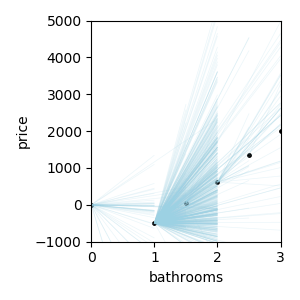
\includegraphics[scale=0.7]{images/baths_vs_price_mipd.png}
\caption{{\bf  Model-independent partial dependence plot of bathrooms versus rent price}}
\label{fig:baths_price_mipd}
\end{center}
\end{figure}

since we care most about how y changes per changes in $x_i$, absolute plots are less useful than relative plots; compare with centered ICE, which I also don't like.

define what we are actually looking for: controlling for other variables or net effect. All other features being equal. partial derivative.

Our approach...

\section{Related work}

There are a few basic approaches to identifying the partial effect of a single variable on the target or response variable:

\begin{itemize}
\item Stratification
\item Beta coefficients from linear model without regularization
\item Marginal plots
\item PDP/ICE
\item Accumulated Local Effects (https://arxiv.org/abs/1612.08468) (ALE) plots
\end{itemize}

PDP math shows that features added or multiplied times the remaining F approximation completely describe the partial dependence; I assume that means that interactions are not a problem.

do we need to talk about LIME?

propensity stuff James mentioned

talk about how we do not presume independence of features
 
This python package seems to do PDP, LIME etc... https://github.com/oracle/Skater

\section{Future work}

This work describes regressors only, ignoring partial dependence for classifiers.  Research reveals no papers or implementation for classifiers. Friedman, however, briefly describes a partial dependence mechanism for classification whereby $k$-class logistic regression (one-versus-rest) equations indicate the probability of seeing class $k$ at $\bf{x}$.  This suffers from the same interaction-based bias as the regressor model.

Actually, the R version of personal dependence may actually do this. See https://christophm.github.io/interpretable-ml-book/pdp.html where he describes PDP for cancer prediction and gets probabilities out.

\section{Conclusion}
\label{sec:conc}

\bibliographystyle{apalike}

\bibliography{stratpd}
\end{document}